\documentclass{article}
\usepackage{graphicx}
\usepackage[margin=1.5cm]{geometry}
\usepackage{amsmath}

\begin{document}
\twocolumn

\title{Monday Warm Up: Unit 1, Current and DC Circuits}
\author{Prof. Jordan C. Hanson}

\maketitle

\section{Memory Bank}

\begin{itemize}
\item $I = \Delta Q / \Delta t$ ... The relationship between current, $I$, and charge.
\item $J = I/A$ ... Current density.
\item $J = \sigma E$ ... Ohm's Law, 1.  $J$ is the current density, and $E$ is the E-field driving current.  The factor $\sigma$ is called the conductivity.  Units: S m$^{-1}$.
\item $\rho = 1/\sigma = E/J$ ... The resistivity.  Units: $\Omega$ m.
\item $V = IR$ ... The macroscopic version of Ohm's law, assuming:
\item $R = L/(\sigma A)$ ... The resistance.  Units: $\Omega$.
\item $R_{\rm tot} = R_1 + R_2$ ... Resistors in series.
\item $R_{\rm tot}^{-1} = R_1^{-1} + R_2^{-1}$ ... Resistors in parallel.
\end{itemize}

\section{Current and DC Circuits}

\begin{enumerate}
\item Consider Fig. \ref{fig:1} (top).  (a) What is the resistance of the circuit implied by the data? (b) What will the current be at 500 V? \\ \vspace{2cm}
\item Consider Fig. \ref{fig:1} (bottom).  (a) If the data was collected from a circuit with two resistors \textit{in series}, what is the value of each resistor? (b) If the data was collected from a circuit with two resistors \textit{in parallel}, what is the value of each resistor? \\ \vspace{4cm}
\item Suppose you have a simple circuit with each element in series, in which the voltage source (a battery, for example) gives a positive increase in voltage $+V$, and each other element $i$ gives $-V_i$.  Based on energy conservation, show that
\begin{equation}
V - V_1 - V_2 - ... = 0
\end{equation} \vspace{2cm}
\item Suppose you have a circuit in which one current $I$ enters a point, and $N$ currents leave ($I_i$).  Based on charge conservation, show that 
\begin{equation}
I - I_1 - I_2 - ... = 0
\end{equation}
\end{enumerate}

\begin{figure}
\centering
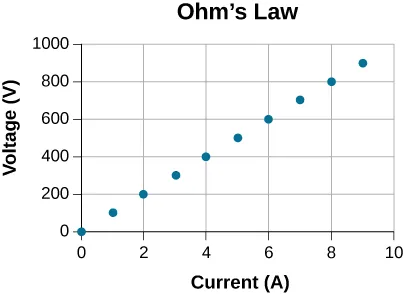
\includegraphics[width=0.33\textwidth]{figures/Ohms.png}
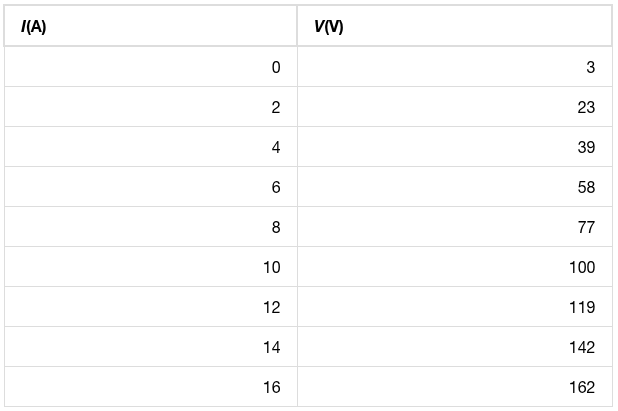
\includegraphics[width=0.4\textwidth]{figures/Ohms2.png}
\caption{\label{fig:1} (Top) The voltage vs. current in a simple DC circuit. (b) The voltage vs. current in a mystery circuit.}
\end{figure}

\end{document}
